\chapter{Práctica: Reconocimiento de la señal Stop}\label{cap.stop}
En este capítulo se expondrá la creación de una nueva práctica para la plataforma de JdeRobot-Academy, llamada ``Reconocimiento de la señal stop''. Se explicará el desarrollo de su infraestructura, su componente académico correspondiente, así como la solución de referencia llevada a cabo. 

\section{Enunciado} \label{sec.enunciado}
El objetivo principal de esta práctica es conseguir que un coche autónomo sea capaz de reconocer una señal de stop. Además, deberá frenar a tiempo en un cruce y después, si no detecta coches, volver a arrancar y realizar un giro a la izquierda o a la derecha de manera aleatoria. El modelo del coche utilizado está dotado de cámaras de vídeo para visualizar el entorno, un sensor de posición y actuadores de movimiento que permiten controlar tanto la velocidad lineal como la de giro. \\

En esta práctica el alumno tiene que programar un algoritmo que cumpla todos los objetivos descritos, evitando que el coche autónomo choque con otros coches u obstáculos de su entorno. En la interfaz gráfica del componente académico se pueden visualizar las imágenes captadas por las cámaras.\\

El algoritmo responde a un control reactivo, por lo que en cada instante actuará en función de los datos captados por los sensores permitiendo controlar el movimiento del coche y reaccionar a distintos imprevistos.

\section{Infraestructura}
En este apartado se describirá el entorno que se ha creado para poder realizar la práctica ``Reconocimiento de la señal stop''. Primero se describirá el modelo del coche utilizado, incluyendo sus sensores y actuadores. Después, se explicará el mundo simulado por el cual se moverá el coche. 

\subsection{Modelo coche Opel}
Para esta práctica se ha creado un nuevo modelo de coche autónomo. El robot está basado en un modelo de coche Opel. Este modelo de coche se denomina \textit{``Opel''} y se puede ver en Figura~\ref{fig.cocheOpel}. Posee tres cámaras de vídeo que se usarán para la detección de la señal de stop y la detección de otros coches; un sensor de posición, que se utilizará para obtener su orientación al realizar los giros, tanto a la izquierda como a la derecha; y motores que le permiten moverse por el mundo de Gazebo.

\begin{figure}[H]
  \begin{center}
    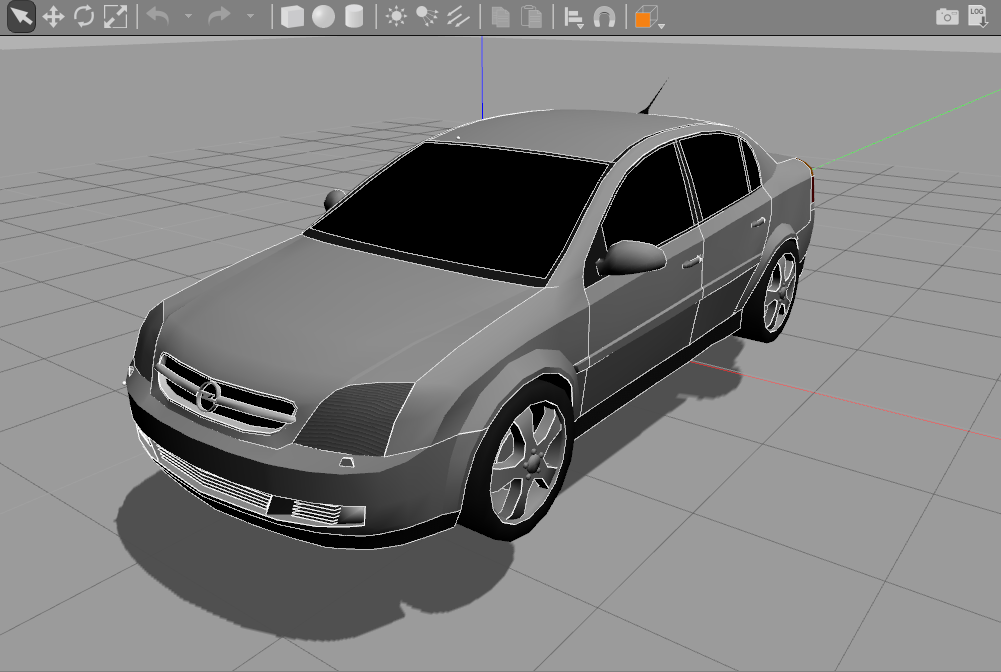
\includegraphics[width=0.7\textwidth]{figures/Stop/cocheOpel.png}
		\caption{Modelo coche Opel}
		\label{fig.cocheOpel}
  \end{center}
\end{figure}

En esta práctica se han empleado los siguientes \textit{plugins} para este modelo:

\begin{itemize}
\item	\textit{OpelMotors}: El componente académico interactúa con este \textit{plugin}. Este \textit{plugin} permite dotar al componente de velocidad, tanto velocidad de tracción como velocidad de rotación.
\item	\textit{camera\_dump}: Este \textit{plugin} será empleado por los componentes para tener visión del entorno.
\item	\textit{Pose3D}: Este \textit{plugin} se emplea para obtener la posición del coche en tiempo real y su orientación.
\end{itemize}


\subsubsection{Cámaras de vídeo}
En este coche se han instalado 3 cámaras de vídeo. Las imágenes captadas tienen un tamaño de 640 x 480 píxeles y están basadas en el modelo de color \acrshort{rgb} (cada uno de estos tres canales esta codificado con 1 byte). El rango de profundidad de visión de las cámaras abarca desde 10 centímetros hasta 35 metros. Una de las cámaras está situada en el centro del techo (ligeramente a la derecha), otra al lado del faro derecho (orientada hacia a la derecha) y la última, a lado del faro izquierdo (orientada hacia a la izquierda). De esta manera, conseguimos un campo de visión más amplio. La cámara central se usará para el proceso de detección de la señal de stop y la carretera, y las cámaras laterales, para la detección de otros coches.

\subsection{Modelo car}
Se han añadido dos coches adicionales que se mueven de manera automática a lo largo de una de las carretera para simular el tráfico de una calle. Ambos coches utilizan la misma malla visual que el modelo Opel por lo que tienen el mismo aspecto. \\

Para conseguir que los coches se muevan de manera automática, se ha creado un nuevo \textit{plugin} llamado \textit{``carplugin''}. Este \textit{plugin} dota de velocidad lineal constante al modelo en su eje x y, dependiendo de su posición en el simulador Gazebo, tomará dirección positiva o negativa.


\subsection{Modelo stop\_sign}
Debido a que el objetivo principal de la práctica es reconocer una señal de stop, se ha añadido el modelo \textit{``stop\_sign''}. Este modelo se puede ver en la Figura~\ref{fig.stopSign}.

\begin{figure}[H]
  \begin{center}
    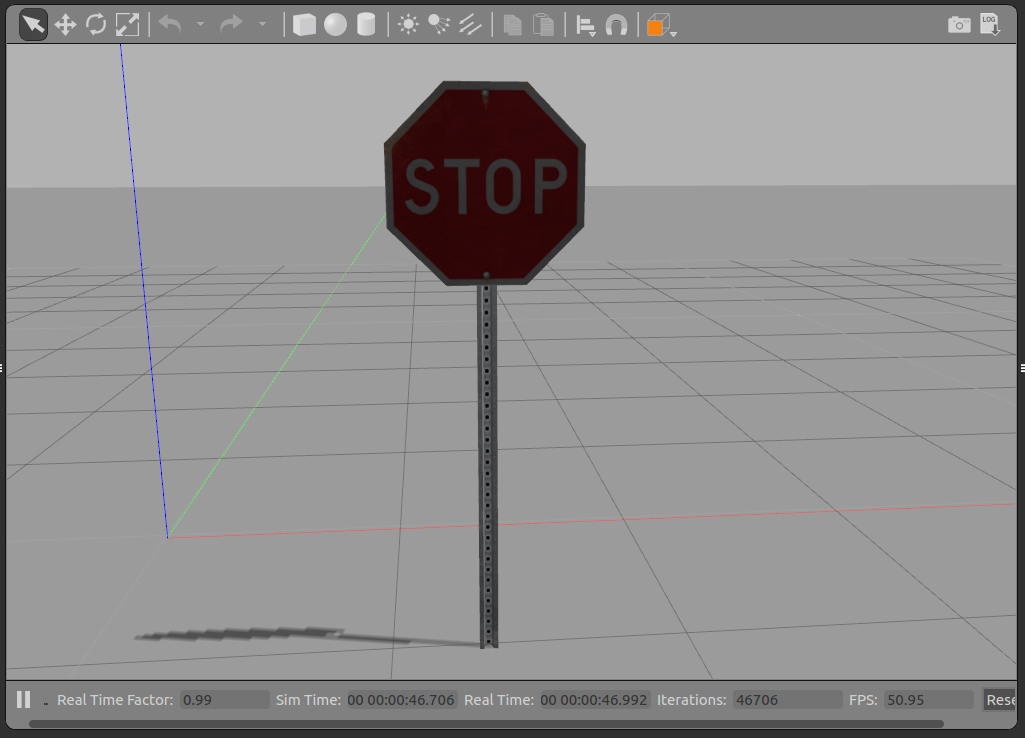
\includegraphics[width=0.5\textwidth]{figures/Stop/stopSign.png}
		\caption{Modelo stop\_sign}
		\label{fig.stopSign}
		\end{center}
\end{figure}

\subsection{Modelo StopW}
Ha sido necesario crear el modelo de un cruce de carreteras por donde circularán los coches utilizados en esta práctica. Este modelo se ha denominado \textit{``StopW''} y se puede ver en la Figura~\ref{fig.stopW}. 

\begin{figure}[H]
  \begin{center}
    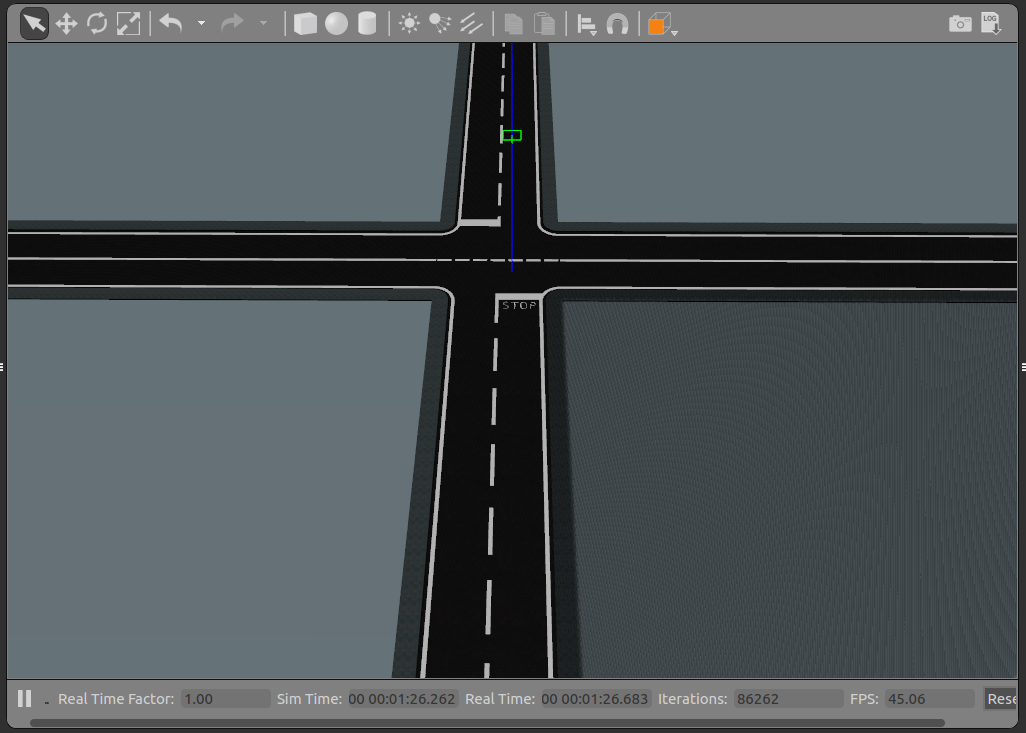
\includegraphics[width=0.8\textwidth]{figures/Stop/stopW.png}
		\caption{Modelo stopW}
		\label{fig.stopW}
		\end{center}
\end{figure}

\subsection{Mundo de Gazebo}
Los mundos que se simulan con Gazebo son mundos 3D. Estos mundos se cargan en ficheros con extensión .world, que no son más que ficheros \acrshort{xml} definidos en el lenguaje \acrshort{sdf}. Este lenguaje contiene una descripción completa de todos los elementos que tiene el mundo y los robots.\\

El mundo creado en Gazebo está formado por un modelo de cruce de carreteras \textit{``stopW''}, dos señales de stop con el modelo \textit{``stop\_sign''}, poseerá 2 coches que se mueven de manera autómatica empleando el modelo \textit{``car''} y se incluirá el modelo del coche \textit{``Opel''}, que ejecutará la solución desarrollada. Por útimo, para dotar de realismo al mundo se han añadido algunos modelos que tiene Gazebo:

\begin{itemize}
\item	Modelo \textit{sun}: Añade una fuente de luz global a la escena.
\item	Modelo \textit{house\_1}, modelo \textit{house\_2}, modelo \textit{house\_3}: Se han utilizado distintos modelos de casas.
\item	Modelo \textit{gas\_station}: Se ha añadido el modelo de una gasolinera.
\item	Modelo \textit{lamp\_post}: Se han añadido un total de 14 farolas situadas a lo largo de las carreteras.
\end{itemize}

Para tener este escenario se ha creado un mundo en Gazebo llamado \textit{``stop.world''}:

\vspace{20pt}
	\begin{lstlisting}[frame=single]
<?xml version="1.0"?>
<sdf version="1.4">
  <world name="default">
  
    <scene>
      <grid>false</grid>
    </scene>
  
    <!-- A global light source -->
    <include>
      <uri>model://sun</uri>
      <pose>1.5 -30 100 0 0 0</pose>
    </include>
    
    <!-- Stop signs -->
    <include>
      <static>true</static>
      <uri>model://gazebo/models/stop_sign</uri>
      <pose>3.5 -3.5 0 0 0 0</pose>
    </include>
    
    <include>
      <static>true</static>
      <uri>model://gazebo/models/stop_sign</uri>
      <pose>-3 3 0 0 0 3.15</pose>
    </include>
    
    
    <!-- Houses -->
    <include>
      <uri>model://house_1</uri>
      <pose>-9.5 8.5 0 0 0 0</pose>
    </include>
    
    <include>
      <uri>model://house_2</uri>
      <pose>-25 7.5 0 0 0 0</pose>
    </include>
    
    <include>
      <uri>model://house_3</uri>
      <pose>-5.5 -7 0 0 0 1.55</pose>
    </include>
    
    
    <!-- A gas station -->
    <include>
      <uri>model://gas_station</uri>
      <pose>10 14 0 0 0 1.55</pose>
    </include>
    
    
    <!-- Lamps -->
    <include>
      <uri>model://lamp_post</uri>
      <pose>-3 13 0 0 0 1.55</pose>
    </include>
    <include>
      <uri>model://lamp_post</uri>
      <pose>3 23 0 0 0 -1.55</pose>
    </include>
    <include>
      <uri>model://lamp_post</uri>
      <pose>-3 33 0 0 0 1.55</pose>
    </include>
    
    <include>
      <uri>model://lamp_post</uri>
      <pose>-3 -3 0 0 0 1.55</pose>
    </include>
    <include>
      <uri>model://lamp_post</uri>
      <pose>3 -13 0 0 0 -1.55</pose>
    </include>
    <include>
      <uri>model://lamp_post</uri>
      <pose>-3 -23 0 0 0 1.55</pose>
    </include>
    <include>
      <uri>model://lamp_post</uri>
      <pose>3 -33 0 0 0 -1.55</pose>
    </include>
    
    <include>
      <uri>model://lamp_post</uri>
      <pose>3 3 0 0 0 0</pose>
    </include>
    <include>
      <uri>model://lamp_post</uri>
      <pose>13 -3 0 0 0 3.15</pose>
    </include>
    <include>
      <uri>model://lamp_post</uri>
      <pose>23 3 0 0 0 0</pose>
    </include>
    <include>
      <uri>model://lamp_post</uri>
      <pose>33 -3 0 0 0 3.15</pose>
    </include>

    <include>
      <uri>model://lamp_post</uri>
      <pose>-13 3 0 0 0 0</pose>
    </include>
    <include>
      <uri>model://lamp_post</uri>
      <pose>-23 -3 0 0 0 3.15</pose>
    </include>
    <include>
      <uri>model://lamp_post</uri>
      <pose>-33 3 0 0 0 0</pose>
    </include>
    

    <!-- A opel car -->
    <include>
      <uri>model://opel</uri>
      <pose>1.5 -30 0 0 0 3.14</pose> 
    </include>
    
    
    <!-- Cars -->
    <include>
      <uri>model://car</uri>
      <pose>-30 -1.5 0 0 0 1.57</pose>
    </include>
    
    <include>
      <uri>model://car</uri>
      <pose>40 1.5 0 0 0 -1.57</pose>
    </include>
    
    
    <!-- Roads -->
    <include>
      <uri>model://stopW</uri>
      <pose>0 0 0 0 0 0</pose>
    </include>
    
  </world>
</sdf>
	\end{lstlisting}


En la Figura~\ref{fig.stopWorld} se puede observar el mundo creado en Gazebo.

\begin{figure}[H]
  \begin{center}
    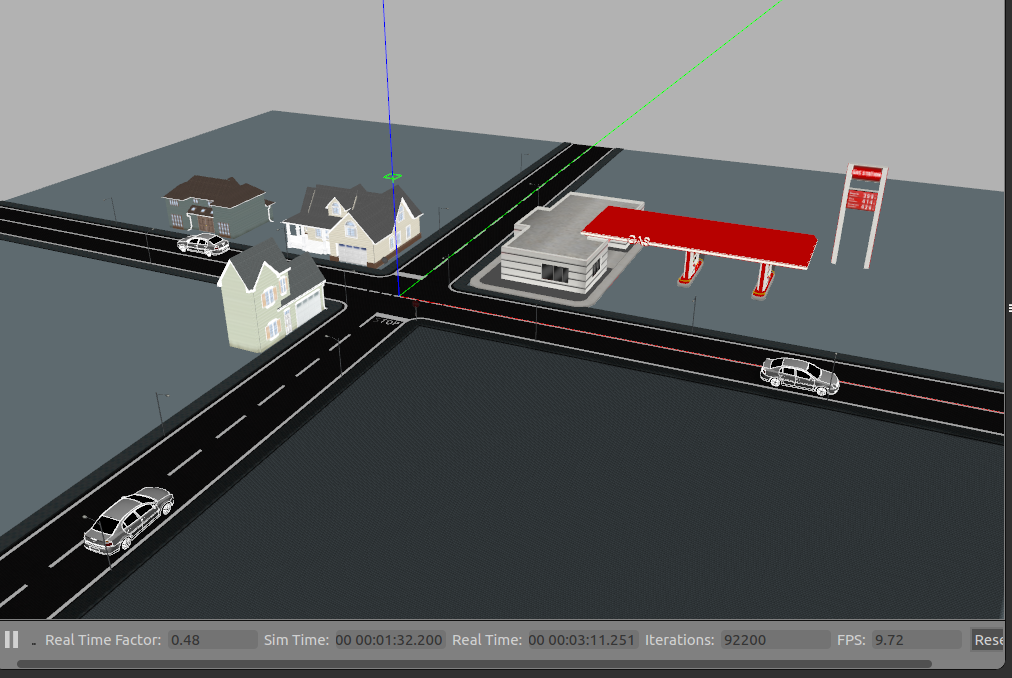
\includegraphics[width=1.0\textwidth]{figures/Stop/stopWorld.png}
		\caption{Mundo stop.world en Gazebo}
		\label{fig.stopWorld}
		\end{center}
\end{figure}


\section{Componente académico}
Se ha creado un componente académico para esta práctica que resuelve diversas funcionalidades: (a) muestra una interfaz gráfica al usuario, con distintos elementos, que permiten depurar el código de manera más sencilla; (b) ofrece acceso a sensores y actuadores en forma de métodos simples ocultando el \textit{middleware} de comunicaciones; (c) incluye código auxiliar que ayuda a programar la solución. El componente deja todo listo para que el estudiante sólo tenga que incorporar su código rellenando el método \textit{execute} en el fichero \textit{MyAlgorithm.py}.\\

Este componente ofrece al programador del algoritmo este \acrshort{api} de sensores y actuadores:

\begin{itemize}
\item 	\textit{pose3d.getX()}: Permite obtener la posición absoluta del robot en el eje X.
\item	\textit{pose3d.getY()}: Permite obtener la posición absoluta del robot en el eje Y.
\item	\textit{pose3d.getYaw()}: Permite obtener la orientación del robot con respecto al sistema de referencia de Gazebo.
\item 	\textit{motors.sendV()}: Para establecer la velocidad lineal.
\item	\textit{motors.sendW()}: Para establecer la velocidad de giro.
\item	\textit{cameraC.getImage()}: Permite obtener las imágenes captadas por la cámara situada en el techo del coche.
\item	\textit{cameraL.getImage()}: Permite obtener las imágenes captadas por la cámara situada en el faro izquierdo.
\item	\textit{cameraR.getImage()}: Permite obtener las imágenes captadas por la cámara situada en el faro derecho.
\end{itemize}

Es necesario crear un archivo de configuración (\textit{stop.cfg}) donde se indican los puertos utilizados por los distintos \textit{plugins}, la velocidad lineal máxima y la velocidad angular máxima de los motores.:

\vspace{20pt}
	\begin{lstlisting}[frame=single]
Stop.CameraC.Proxy  = cam_opel_center:default -h localhost -p 8995
Stop.CameraL.Proxy  = cam_opel_left:default -h localhost -p 8996
Stop.CameraR.Proxy  = cam_opel_right:default -h localhost -p 8997
Stop.Motors.Proxy  = Motors:default -h localhost -p 9999
Stop.Pose3D.Proxy  = Pose3D:default -h localhost -p 9989

Stop.Motors.maxV = 250
Stop.Motors.maxW = 20
	\end{lstlisting}

En esta práctica, los motores emplean el puerto 9999; el sensor de posición el puerto 9989; y las cámaras central, izquierda y derecha utilizan los puertos 8995, 8996 y 8997, respectivamente. \\

Para poder realizar todas las tareas necesarias para el funcionamiento de la práctica se emplean dos hilos de ejecución:

\begin{itemize}
\item	Hilo de control: se encarga de actualizar de manera constante los datos captados por los sensores y los datos enviados a los actuadores. Debido a que se trata de una solución reactiva es necesario que el intervalo de actualización de dichos datos sea un tiempo muy corto, en este caso, 50 ms. Si se fijara un tiempo muy grande podría ocasionar errores en la trayectoria del robot.
\item	Hilo de la \acrshort{gui}: este hilo actualiza la interfaz gráfica que se muestra al usuario. Este intervalo de actualización debe de ser también corto ya que la interfaz gráfica es una herramienta que utiliza el programador para depurar su código y debe de mostrar de manera fiable los datos del robot en tiempo real. Este intervalo también es de 50 ms.
\end{itemize}


\subsection{Interfaz gráfica}
Para que la realización de la práctica sea más fácil, se ha creado una interfaz gráfica que muestra datos importantes, relativos al robot, al usuario. Además, esta interfaz permite de manera sencilla ejecutar el código donde se desarrolla la solución correspondiente. Se ha empleado la herramienta PyQt5 para su desarrollo.\\

En la parte izquierda de la interfaz gráfica, se muestran las imágenes captadas por las tres cámaras de vídeo instaladas en el robot. Mediante estas imágenes el programador podrá verificar si está realizando correctamente el tratamiento digital de las imágenes necesario para detectar tanto la señal de stop, como la carretera o los otros coches. Las imágenes de la cámara izquierda se reproducen a la izquierda de la interfaz, las de la cámara central en el centro y las de la cámara derecha a la derecha.\\

A la derecha, hay un teleoperador que permite mover el coche manualmente. Se puede controlar tanto la velocidad lineal (en el eje vertical) como la velocidad de giro (eje horizontal). \\

En la parte inferior, aparecen dos botones. El botón situado bajo las imágenes captadas por las cámaras, permite tanto ejecutar como parar el código alojado en el archivo \textit{MyAlgorithm.py}. Con el botón que está bajo el teleoperador, se puede detener al robot si se está controlando con el teleoperador. \\

En la Figura~\ref{fig.stopGUI} se muestra el resultado de la interfaz gráfica que verá el usuario en todo momento.

\begin{figure}[H]
  \begin{center}
    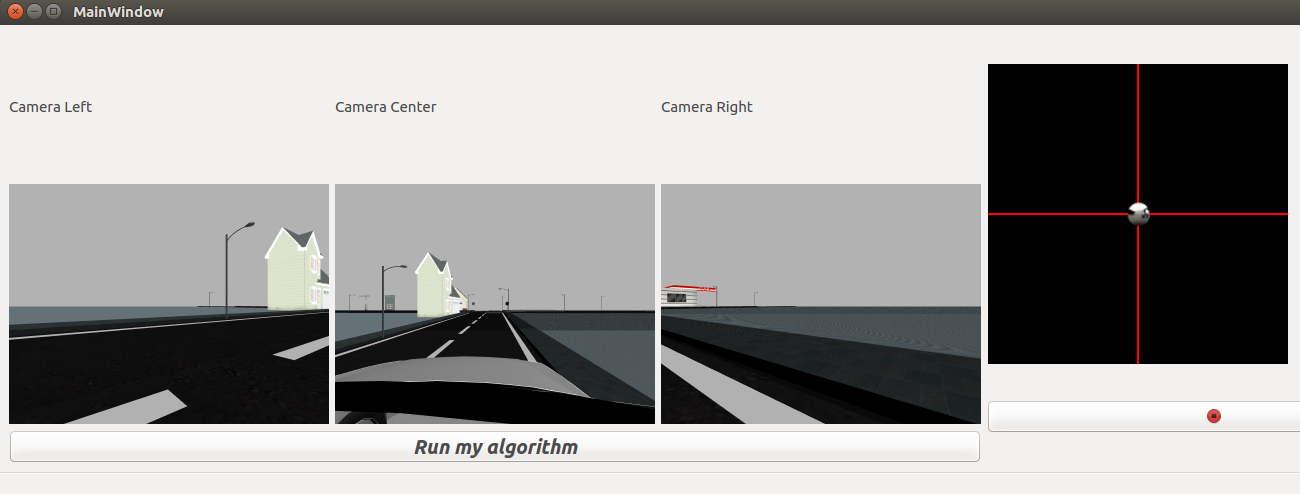
\includegraphics[width=1.0\textwidth]{figures/Stop/stopGUI.png}
		\caption{Interfaz gráfica}
		\label{fig.stopGUI}
		\end{center}
\end{figure}


\section{Solución de referencia}
La solución desarrollada para esta práctica resuelve el problema planteado de reconocer una señal de stop. La solución se ha programado en el fichero \textit{MyAlgorithm.py}, en el método \textit{``execute''}, que es el método principal de la solución. De este modo se puede crear un control reactivo, donde el coche irá tomando decisiones según los datos que vaya obteniendo de los sensores en tiempo real. Para esta práctica se ha realizado el pilotaje del robot sin una planificación de movimiento previa.\\

La solución puede dividirse en tres partes principales: (a) reconocimiento de la señal de stop y frenado del coche; (b)detección de otros coches; (c) realización del giro. 

\subsection{Reconocimiento de la señal de stop y frenado del coche}
Para detectar la señal de stop, nos basaremos en dos de sus características principales: el color y la forma. Si solo nos centráramos en el color podría llevarnos a error, ya que existen más señales viales de color rojo, por lo que necesitamos fijarnos en otra característica. En este caso nos hemos decantado por la forma ya que la señal de stop es la única señal vial que tiene forma octogonal. \\

Para llevar acabo el proceso de detección, utilizaremos las imágenes captadas por la cámara situada en el techo del coche. A estas imágenes les aplicamos un filtro de color para detectar el color rojo específico de la señal. Para ello, hemos creado la función \textit{``filterHSV''} que realizará el cambio de modelo de color de \acrshort{rgb} (Figura~\ref{fig.imgRGByHSV}) al modelo \acrshort{hsv}, el proceso de segmentación (Figura~\ref{fig.colorFilterRed}) y aplicará la operación morfológica de cierre (Figura~\ref{fig.close}) para eliminar la palabra ``STOP'' de la señal. Para fijar los valores del filtro, hemos utilizado la herramienta ``colorTuner'' de JdeRobot.\\

\begin{figure}[H]
  \begin{center}
    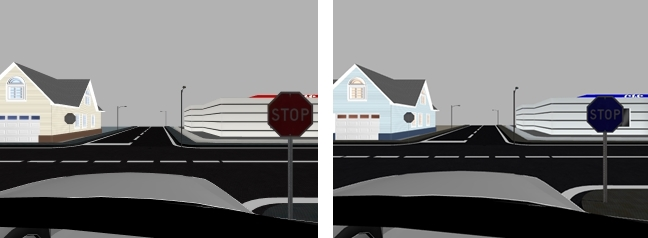
\includegraphics[width=0.8\textwidth]{figures/Stop/imgRGByHSV.jpg}
		\caption{Imagen original en RGB y en HSV}
		\label{fig.imgRGByHSV}
		\end{center}
\end{figure}

\begin{figure}[H]
  \begin{center}
    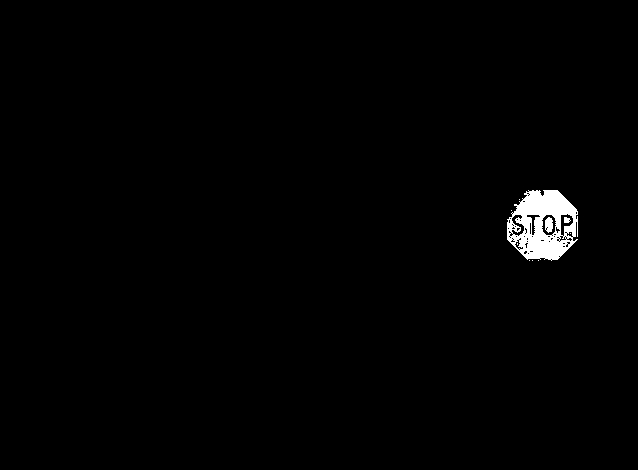
\includegraphics[width=0.5\textwidth]{figures/Stop/colorFilterRed.jpg}
		\caption{Imagen con filtro de color rojo}
		\label{fig.colorFilterRed}
		\end{center}
\end{figure}

\begin{figure}[H]
  \begin{center}
    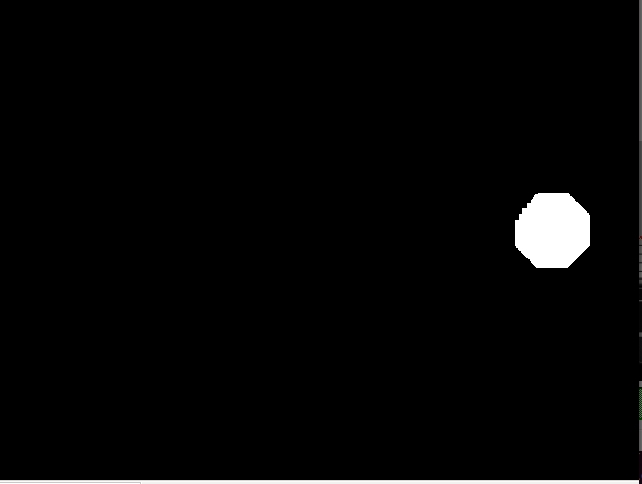
\includegraphics[width=0.5\textwidth]{figures/Stop/close.jpg}
		\caption{Imagen con cierre}
		\label{fig.close}
		\end{center}
\end{figure}


De esta manera, obtenemos una imagen binaria con la forma de la señal de stop en primer plano (blanco) (Figura~\ref{fig.close}). Esta imagen la compararemos con una plantilla de referencia para comprobar que se trata de la forma que queremos (octogonal). Para realizar esta comparación recortamos la imagen filtrada (Figura~\ref{fig.cut}) para quedarnos solo con la parte de la imagen que contiene la señal y la redimensionamos para que, tanto esta imagen como la plantilla (Figura~\ref{fig.template}), tengan el mismo tamaño y poder realizar correctamente el cotejamiento. \\

\begin{figure}[H]
  \begin{center}
    
\includegraphics[width=0.2\textwidth]{figures/Stop/cut.jpg}
		\caption{Señal de stop recortada}
		\label{fig.cut}
		\end{center}
\end{figure}

\begin{figure}[H]
  \begin{center}
    
\includegraphics[width=0.2\textwidth]{figures/Stop/template.png}
		\caption{Plantilla de referencia}
		\label{fig.template}
		\end{center}
\end{figure}

Una vez que hemos detectado la señal, el coche deberá frenar hasta situarse en el cruce de las dos carreteras. Para realizar el frenado hemos creado la función \textit{``brake''}, mediante la cual, el coche irá reduciendo su velocidad lineal según el tamaño que vaya adquiriendo la señal de stop detectada. Al principio, esta señal será pequeña ya que estará a lo lejos e irá aumentando de tamaño según el coche se vaya acercando hacia ella (Figura~\ref{fig.brake}). Para saber el tamaño de la señal, realizamos un \textit{bounding} alrededor de la señal (Figura~\ref{fig.stopRecuadro}) y, según el tamaño del recuadro, se llevarán a cabo las distintas fases del frenado, disminuyendo paulatinamente la velocidad. \\

\begin{figure}[H]
  \begin{center}
    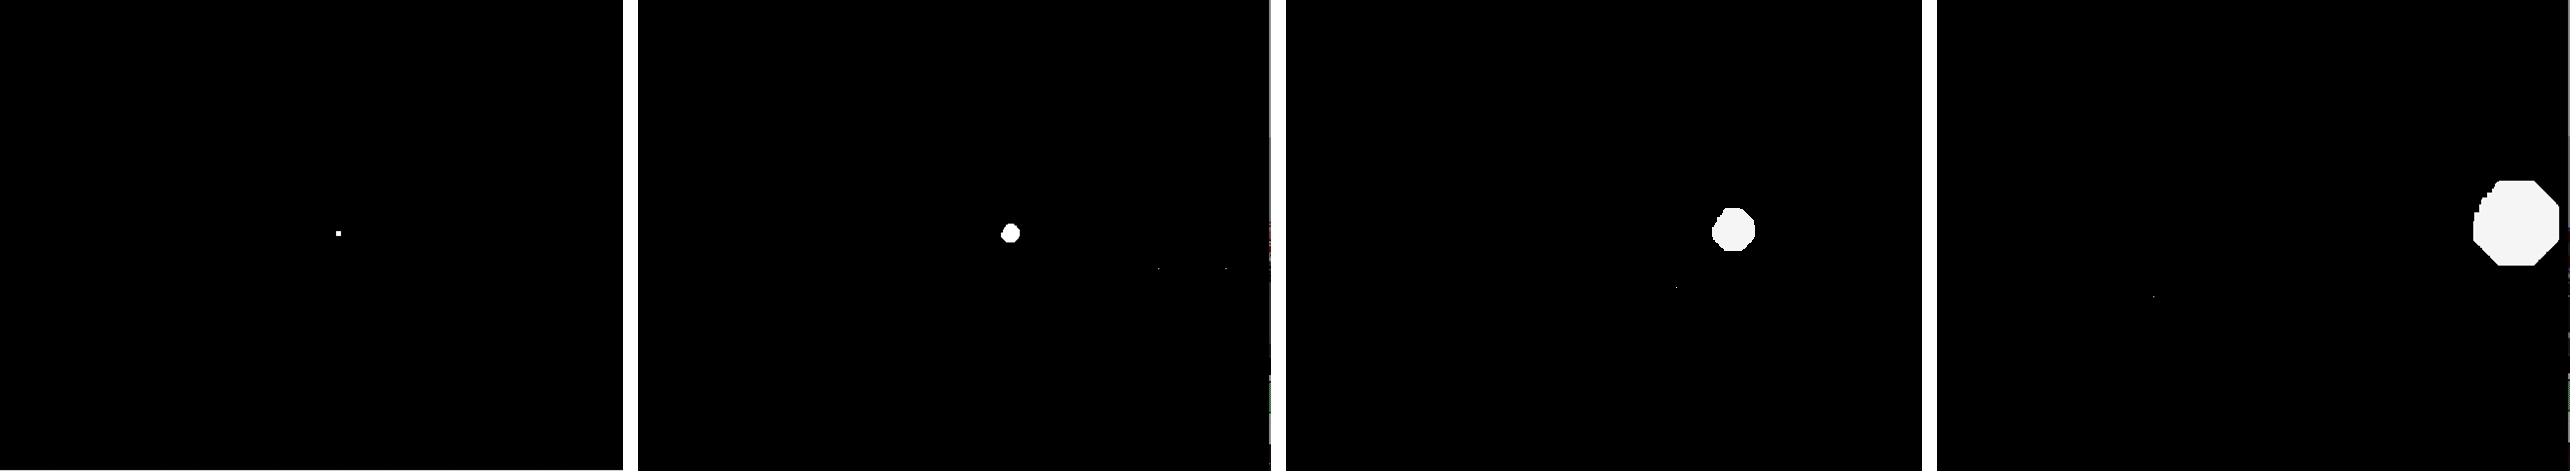
\includegraphics[width=1.0\textwidth]{figures/Stop/brake.jpg}
		\caption{Aumento del tamaño de la señal de stop}
		\label{fig.brake}
		\end{center}
\end{figure}

\begin{figure}[H]
  \begin{center}
    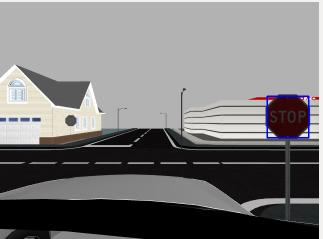
\includegraphics[width=0.5\textwidth]{figures/Stop/stopRecuadro.jpg}
		\caption{Señal de stop recuadrada}
		\label{fig.stopRecuadro}
		\end{center}
\end{figure}

\subsection{Detección de otros coches}
Después de frenar, el coche deberá saber si vienen o no otros vehículos y luego reanudar su camino. Para distinguir a los otros coches que circulan por la carretera perpendicular, nos basamos en la resta de imágenes para detectar su movimiento (ya que en este escenario serán los únicos elementos que se moverán). Usaremos las imágenes captadas por las cámaras situadas en los faros de los coches (tanto la izquierda como la derecha), las transformaremos a escala de grises y les aplicaremos un suavizado mediante un filtro de Gauss para que la detección de movimiento sea más sencilla (Figura~\ref{fig.imgL}). Hemos creado la función \textit{``motionDetection''} que se encargará de calcular la diferencia entre los distintos fotogramas; aplicar un umbral para segmentar la imagen y solo quedarnos con las zonas de mucho movimiento (puede que existan vibraciones en las imágenes debido a la inercia del robot y este movimiento no nos interesa); y dilatar la imagen resultante para intentar eliminar el mayor número de partes negras dentro del coche detectado (Figura~\ref{fig.motionDetection}). Realizamos la resta de fotogramas con una diferencia de 5 fotogramas entre el actual y el anterior. 

\begin{figure}[H]
  \begin{center}
    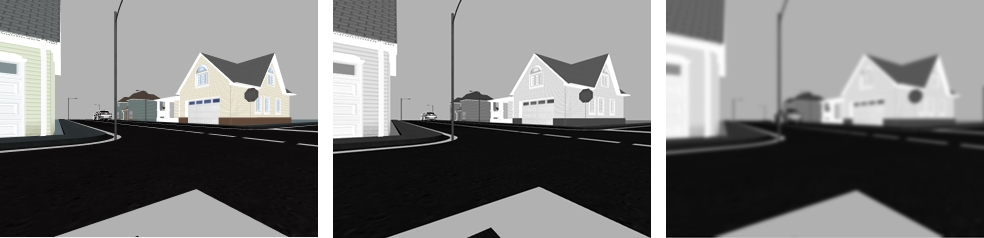
\includegraphics[width=1.0\textwidth]{figures/Stop/imgL.jpg}
		\caption{Imagen original, en escala de grises y suavizada}
		\label{fig.imgL}
		\end{center}
\end{figure}

\begin{figure}[H]
  \begin{center}
    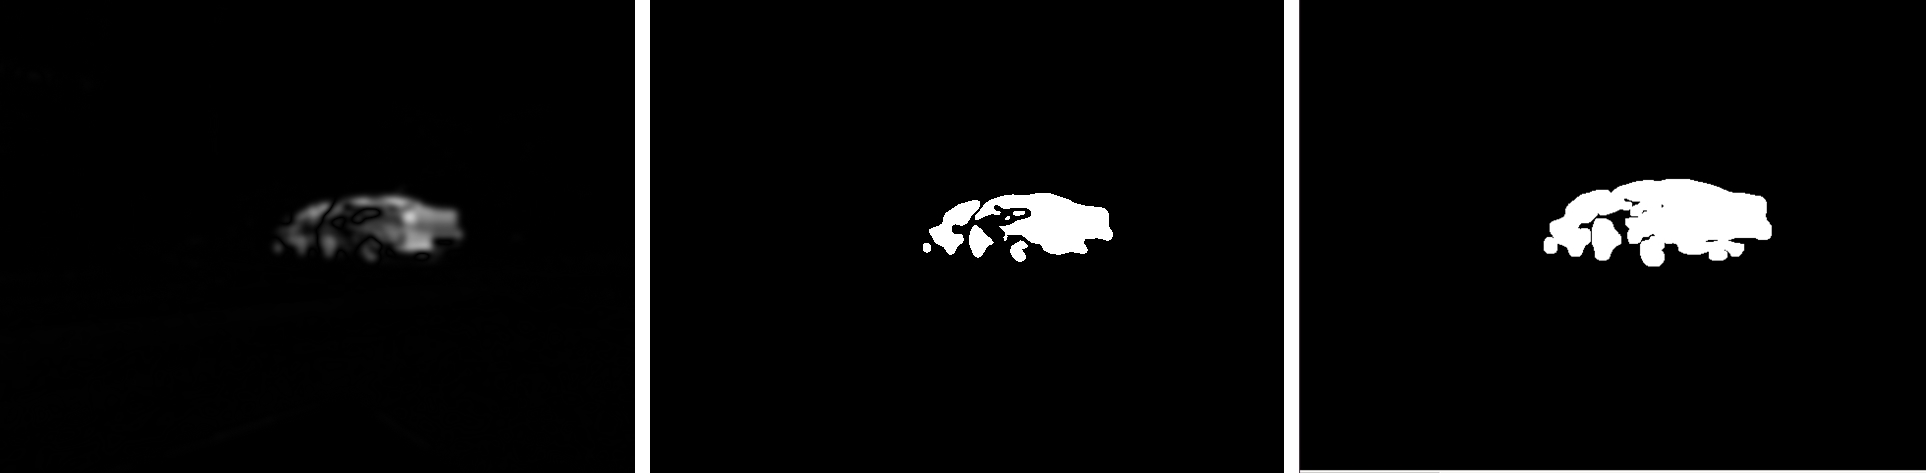
\includegraphics[width=1.0\textwidth]{figures/Stop/motionDetection.jpg}
		\caption{Proceso de detección de movimiento}
		\label{fig.motionDetection}
		\end{center}
\end{figure}

\subsection{Realización del giro}
Para decidir si el coche comienza o no a moverse de nuevo hemos creado la variable dinámica \textit{``detectionCar''}. Ésta irá disminuyendo su valor a lo largo del tiempo y aumentará si se detectan coches mediante la función \textit{``findCar''}. Cuando esta variable sea menor que el umbral establecido, el coche considerará que ha pasado un tiempo razonable sin detectar a otros vehículos y reanudará su ruta. \\

Ahora, el coche deberá girar a la izquierda o a la derecha. La dirección del giro se escogerá de manera aleatoria mediante la función creada \textit{chooseDir}. Una vez elegida la dirección el coche llevará a cabo un giro de 45º y después comenzará a detectar la carretera para situarse en el centro del carril derecho. Para realizar la detección de la carretera utilizaremos de nuevo la cámara situada en el techo del coche. A las imágenes captadas volveremos a aplicarles la función \textit{``filterHSV''} pero esta vez los valores del filtro serán los correspondientes al color gris de la carretera (Figura~\ref{fig.road}). Para seleccionar estos valores también utilizamos la herramienta ``colorTuner'' de JdeRobot.\\

\begin{figure}[H]
  \begin{center}
    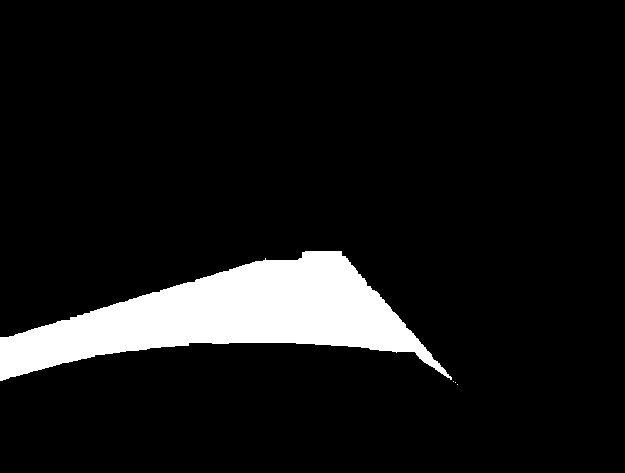
\includegraphics[width=0.5\textwidth]{figures/Stop/road.jpg}
		\caption{Carretera filtrada}
		\label{fig.road}
		\end{center}
\end{figure}

Una vez hemos realizado el filtrado de color de la imagen y hemos obtenido la carretera en primer plano, necesitamos hallar los límites de la carretera para que, posteriormente, el coche sea capaz de posicionarse correctamente en el carril derecho. Para ubicar los bordes, hemos creado la función \textit{``findRoad''} que recorrerá las columnas de la imagen y buscará los cambios de color que aparezcan en la fila 300 de la imagen. Hemos elegido esta fila para asegurar que contenga a la carretera (que estará en la parte inferior de la imagen). Si los píxeles cambian de negro a blanco se tratará del borde izquierdo y si cambian de blanco a negro se tratará del borde derecho. Después, deberemos encontrar la mitad de la carretera ya que marcará la separación de los dos carriles, y posteriormente, hallaremos la mitad del carril derecho (Figura~\ref{fig.desv}). Estas operaciones las llevará a cabo la función creada \textit{``findMidLane''}. \\

\begin{figure}[H]
  \begin{center}
    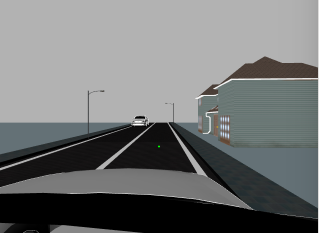
\includegraphics[width=0.5\textwidth]{figures/Stop/desv.png}
		\caption{Punto central del carril derecho de color verde}
		\label{fig.desv}
		\end{center}
\end{figure}

Para saber si el coche está circulando por el carril adecuado, haremos un control del pilotaje basándonos en la desviación que haya entre el centro de la imagen y el punto que marca el centro del carril derecho. Para ello, hemos creado la función \textit{``controlDesviation''} que aplicará una velocidad de giro a los motores directamente proporcional al valor de la desviación del vehículo en el carril por el que circula. También tendrá en cuenta el signo de la desviación ya que indica hacia qué lado se esta moviendo el coche. Si es negativa, se estará desviando hacia la derecha por lo que tendremos que corregir girando a la izquierda, y si es positiva, haremos el giro a la derecha. Si la desviación es pequeña, el coche simplemente irá recto sin girar.

\section{Experimentación}

\subsection{Ejecución típica} 
Para ejecutar esta práctica, es necesario abrir dos terminales y ejecutar los siguientes comandos:

\begin{enumerate}[1.]
\item Lanzar el simulador Gazebo:
	\begin{lstlisting}[frame=single]
		gazebo stop.world
	\end{lstlisting} 
	\begin{enumerate}[1b.]
	\item Se puede arrancar solo el simulador sin la interfaz gráfica:
		\begin{lstlisting}[frame=single]
		 	gzserver stop.world
		\end{lstlisting}
	\end{enumerate}
\end{enumerate}

\begin{enumerate}[2.]
\item	Ejecutar la práctica y lanzar la interfaz gráfica (\acrshort{gui}): 
	\begin{lstlisting}[frame=single]
		python2 stop.py -- --Ice.Config=stop.cfg
	\end{lstlisting} 
\end{enumerate}

En la Figura~\ref{fig.ejecucionFinal} se puede observar como, ejecutando el algoritmo explicado anteriormente, el coche es capaz de frenar cuando reconoce la señal de stop y después, en este caso, realizar el giro hacia la derecha. \\

\begin{figure}[H]
  \begin{center}
    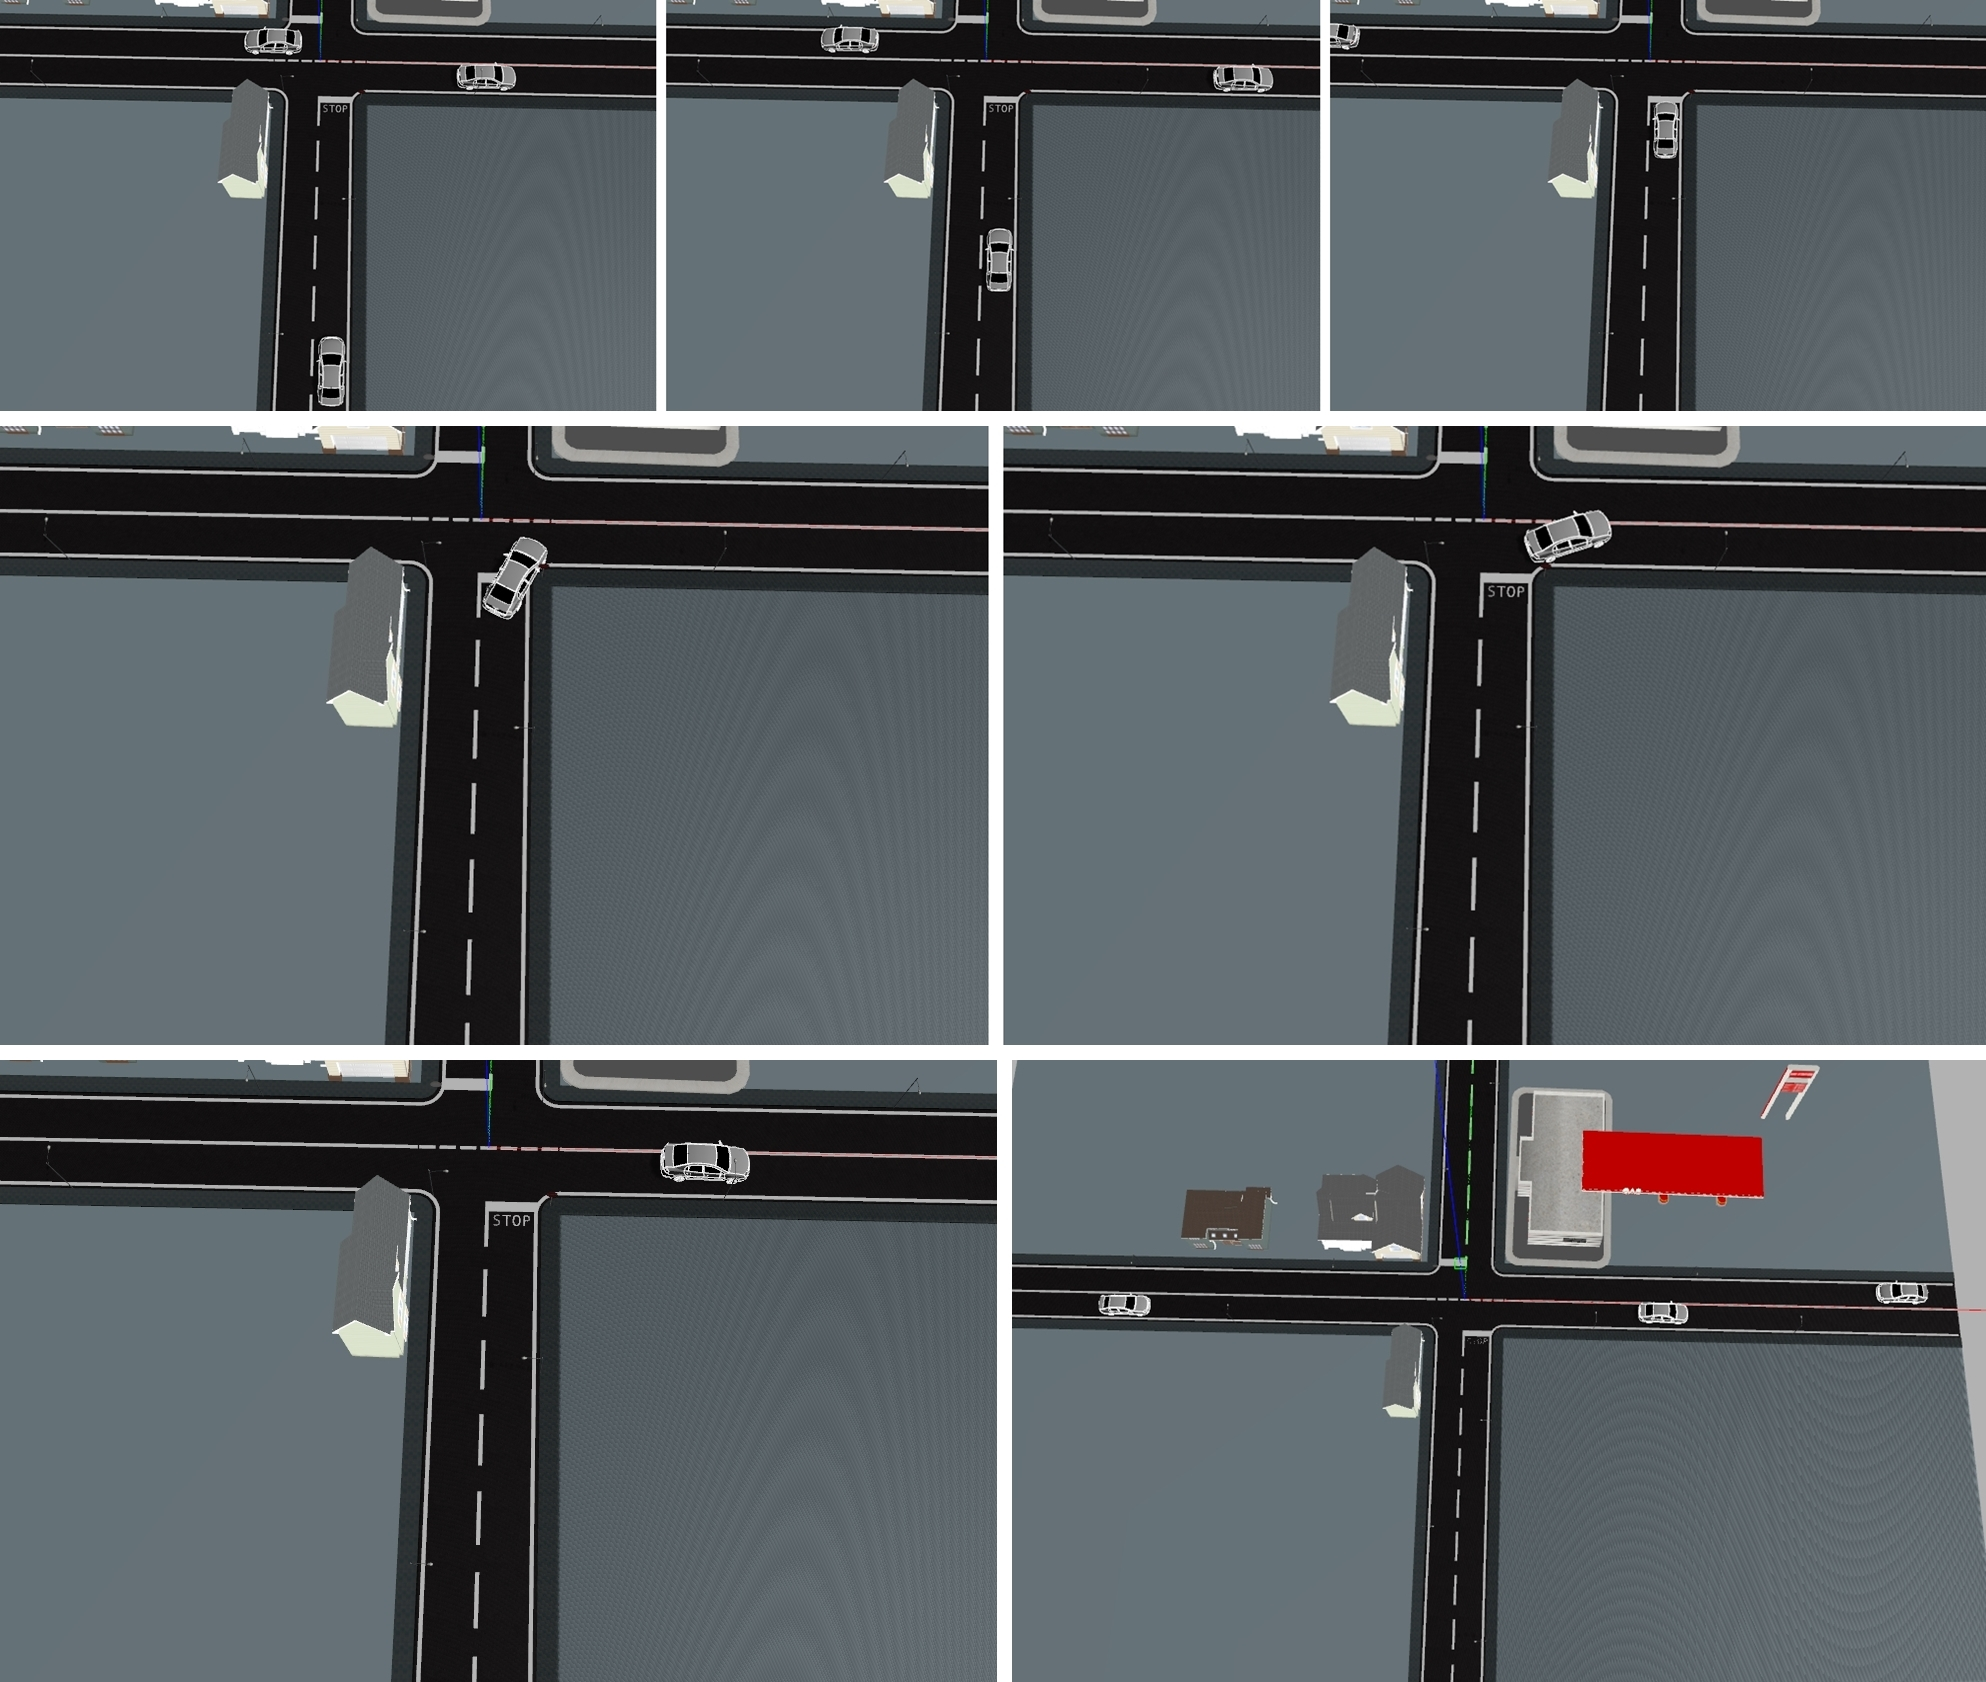
\includegraphics[width=0.9\textwidth]{figures/Stop/ejecucionFinal.jpg}
		\caption{Ejecución típica (giro a la derecha)}
		\label{fig.ejecucionFinal}
		\end{center}
\end{figure}


Una ejecución típica con el giro hacia la izquierda se puede ver en este vídeo \footnote{\url{https://www.youtube.com/watch?v=hF2i0rdlIqE}} y con el giro a la derecha en este otro \footnote{\url{https://www.youtube.com/watch?v=VXZtfHTGsW4}}.
